%% Relatório parcial (draft 1) — baseado no modelo bare_jrnl.tex (IEEEtran V1.8b, Michael Shell).
%% Compilar a partir desta pasta:  pdflatex main && pdflatex main
%% As figuras são geradas por figures/make_figures.py a partir dos resultados em results/.
\documentclass[journal,onecolumn]{IEEEtran}

\usepackage[utf8]{inputenc}
\usepackage[T1]{fontenc}
\usepackage[brazil]{babel}
\usepackage{graphicx}
\usepackage{booktabs}
\usepackage{multirow}
\usepackage{array}
\usepackage{amsmath}
\usepackage{amssymb}
\usepackage{xcolor}
\usepackage{tikz}
\usetikzlibrary{arrows.meta,positioning,fit}
\usepackage{cite}
\usepackage{url}
\usepackage[hidelinks]{hyperref}

\graphicspath{{figures/}}
\newcolumntype{L}[1]{>{\raggedright\arraybackslash}p{#1}}
\newcommand{\Ir}{I_r}
\newcommand{\Ia}{I_a}

\hyphenation{Grounding ViDDAR VIM-Sense}
\renewcommand{\IEEEkeywordsname}{Palavras-chave}

\begin{document}

\title{Robustez de Detectores de Segurança em RA sob Condições Realistas\\
\large Draft 2}

\author{Lucas~Natan~Correia~Couri
        e~Heitor~Mendes~Pereira%
\thanks{Centro de Informática, Universidade Federal de Pernambuco (CIn/UFPE).
E-mails: lncc2@cin.ufpe.br, hmp@cin.ufpe.br.}%
\thanks{Código e documentação: \url{https://github.com/lucascouri2/viddar_rep}.}}

\markboth{Draft 2}{Couri e Pereira: Robustez de detectores de segurança em RA}

\maketitle

\begin{abstract}
Sistemas baseados em modelos de visão e linguagem (VLMs) foram propostos para detectar conteúdo de
realidade aumentada (RA) prejudicial ao usuário, como objetos virtuais que obstruem sinalização real
ou que distorcem o significado de objetos reais. Esses sistemas foram avaliados apenas em dados
curados, sem exposição a degradação realista do ambiente. Nossa hipótese é que placas de sinalização
fisicamente degradadas (desgaste, pichação, adesivos, dano estrutural) podem ser confundidas com
ataques, gerando falsos positivos. Este relatório parcial descreve (i) como usaremos o ViDDAR, um dos
sistemas-base, para testar essa hipótese; (ii) a reconstrução do pipeline de avaliação do ViDDAR, cujo
código publicado era incompleto; (iii) a replicação dos
resultados do artigo original; e (iv), como novidade deste segundo rascunho, a caracterização do conjunto de
dados vwise disponibilizado para o projeto. Esse conjunto não é um dataset de placas: são trechos de
vídeos de direção, rotulados por tipo de ambiente, que incluem vários exemplos gravados
fora da América Latina. O detector de placas do pipeline encontra placas em no máximo cerca de um
quarto dos trechos, em geral pequenas e pouco nítidas, em idiomas variados e sem degradação física
evidente. A hipótese, como formulada, não pode ser testada com esses dados sem complementá-los;
discutimos alternativas viáveis.
\end{abstract}

\begin{IEEEkeywords}
Realidade aumentada, modelos de visão e linguagem, segurança, falsos positivos, robustez, replicação.
\end{IEEEkeywords}

\IEEEpeerreviewmaketitle

% =====================================================================================================
\section{Introdução}

\IEEEPARstart{O}{} conteúdo virtual em RA pode prejudicar a tarefa do usuário quando é mal posicionado
ou mal projetado. O ViDDAR~\cite{viddar} e o VIM-Sense~\cite{vimsense} usam VLMs para detectar dois
tipos de conteúdo prejudicial: \emph{obstrução}, quando o conteúdo virtual esconde um objeto real
importante, e \emph{manipulação de informação}, quando ele induz o usuário a interpretar errado um
objeto real. Ambos comparam a cena real, sem RA, com a cena aumentada.

Os dois sistemas foram avaliados em dados coletados em condições controladas, sem ruído sistemático de
sinalização física degradada. A proposta deste trabalho é medir se placas realisticamente degradadas,
usando os dados indicados pelo professor, fazem esses detectores sinalizarem
ataques inexistentes. O problema tem paralelo na literatura de robustez em visão computacional, com
benchmarks de corrupção de imagem~\cite{hendrycks2019} e exemplos adversariais
naturais~\cite{hendrycks2021}, e no fato conhecido de que adesivos em placas reais já bastam para
enganar classificadores~\cite{eykholt2018}. Até onde sabemos, o efeito ainda não foi estudado em
detectores de segurança para RA.

Nesta primeira etapa escolhemos o ViDDAR como sistema principal, porque ele opera sobre pares de
imagens estáticas. Este relatório cobre:
\begin{itemize}
\item a metodologia proposta para usar o ViDDAR no teste da hipótese (Seção~\ref{sec:metodo});
\item a reconstrução do pipeline de avaliação do ViDDAR (Seção~\ref{sec:impl});
\item a replicação do baseline e seus resultados (Seção~\ref{sec:exp});
\item a caracterização dos dados disponibilizados para o projeto: volume,
  conteúdo, rótulos, origem, localidade, condições de captura, quantidade de placas e um piloto do
  ViDDAR sobre esses dados (Seção~\ref{sec:dados});
\item a discussão do que os resultados implicam para a proposta, incluindo a viabilidade de
  executá-la com esses dados, limitações e questões em aberto (Seções~\ref{sec:disc}
  a~\ref{sec:aberto}).
\end{itemize}

% =====================================================================================================
\section{O sistema-base ViDDAR}
\label{sec:viddar}

O ViDDAR recebe um par de imagens do mesmo ponto de vista: a imagem crua da câmera, $\Ir$, e a imagem
aumentada vista pelo usuário, $\Ia$. A Fig.~\ref{fig:arch} mostra suas duas variantes.

\begin{figure}[!t]
\centering
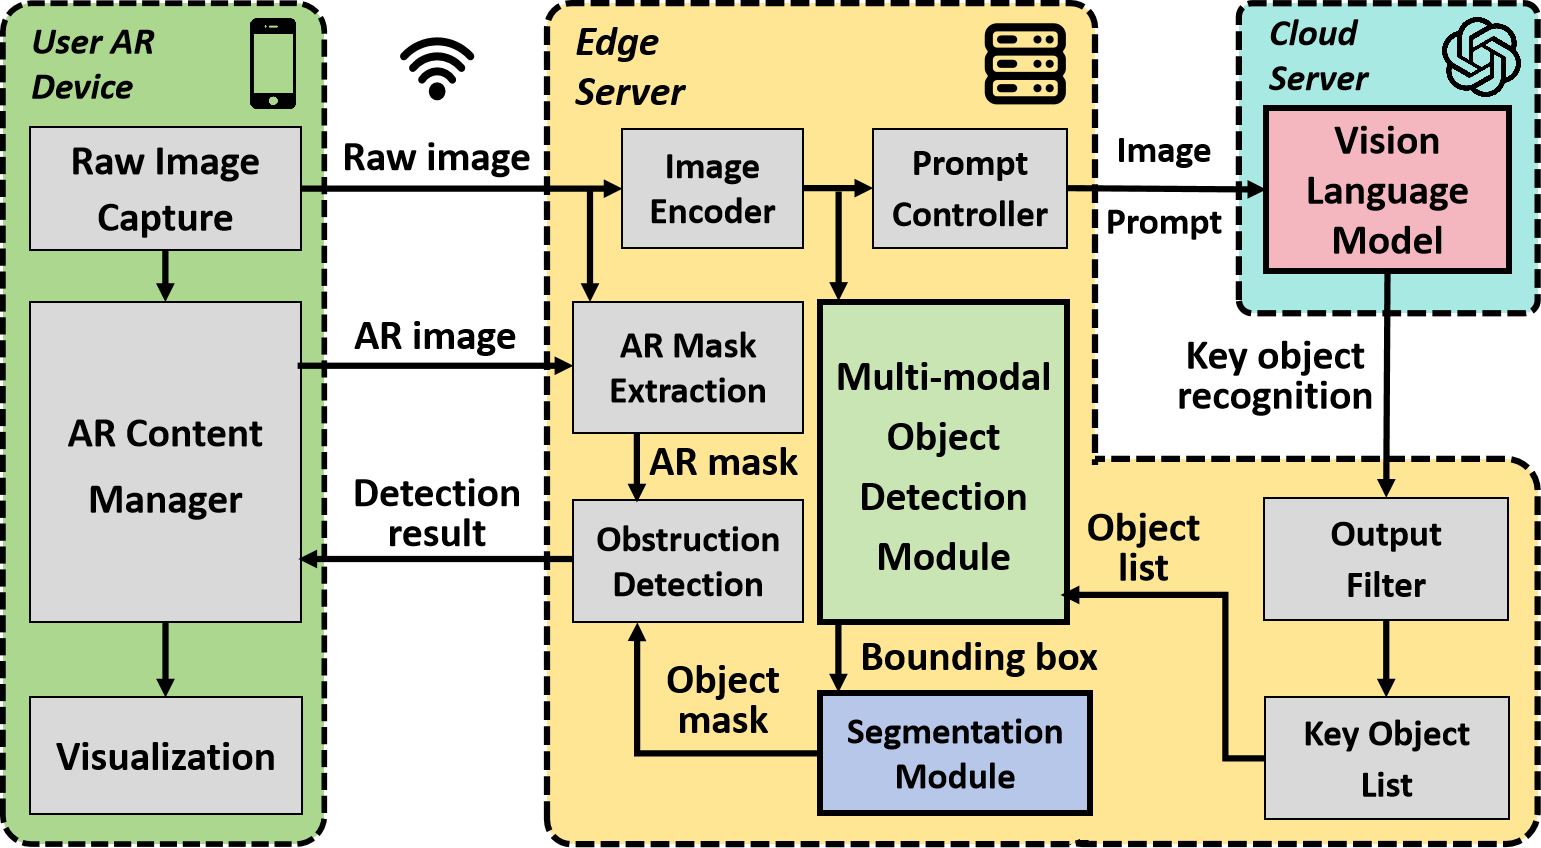
\includegraphics[height=4.3cm]{diagram_obstruction.png}\hfill
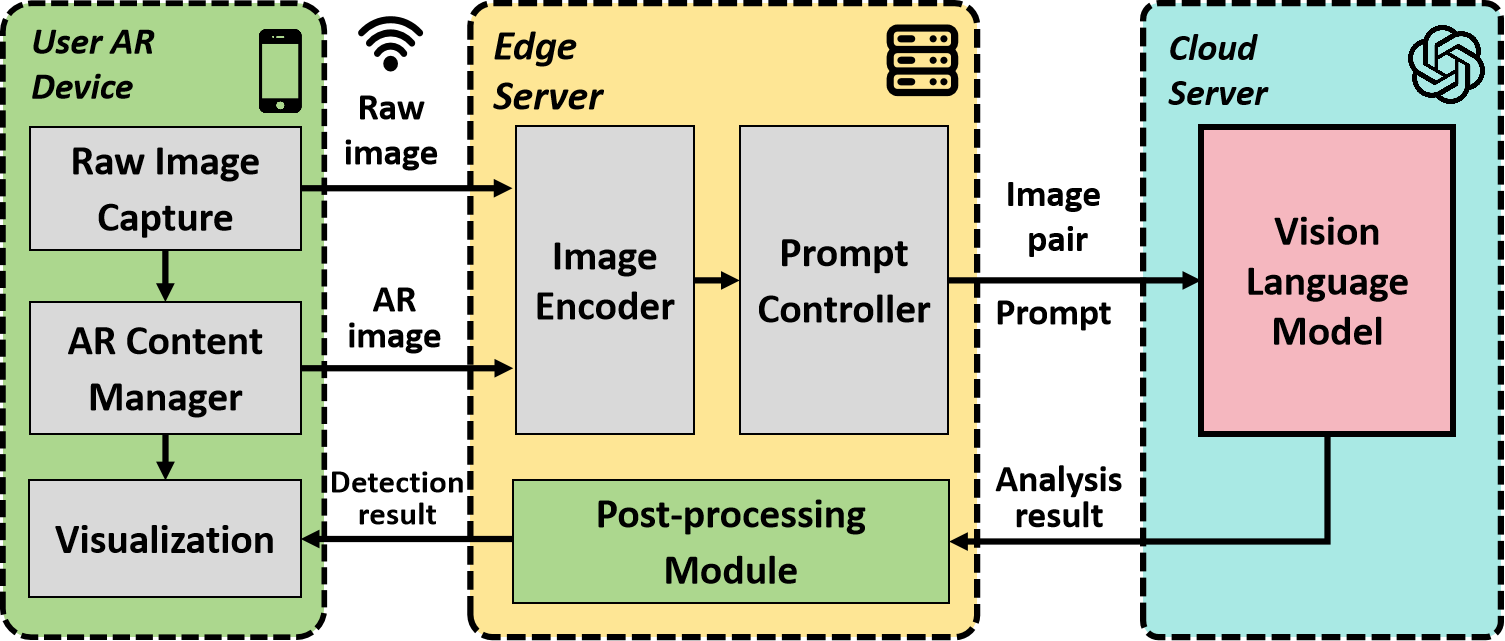
\includegraphics[height=4.3cm]{diagram_information_manipulation.png}
\caption{Arquitetura do ViDDAR para detecção de obstrução (esquerda) e de manipulação de informação
(direita), distribuída entre dispositivo de RA, servidor de borda e nuvem. Fonte: Xiu
\emph{et al.}~\cite{viddar}.}
\label{fig:arch}
\end{figure}

\subsection{Obstrução}
Em $\Ir$ existe um conjunto de objetos-chave $K=\{k_1,\dots,k_n\}$, não predefinido: um objeto é
importante ou não conforme o contexto da cena. Cada $k_i$ tem uma máscara $m_k^i$, e o conteúdo
virtual tem uma máscara $m_c$. Há ataque de obstrução quando
\begin{equation}
O(\Ir,\Ia)=1 \iff \exists\, k_i \in K:\; |m_k^i \cap m_c| \geq \alpha\,|m_k^i|, \qquad \alpha = 0{,}25.
\label{eq:obs}
\end{equation}
O pipeline tem quatro passos:
\begin{enumerate}
\item um VLM recebe $\Ir$ e um prompt com atribuição de papel, exemplos e restrição de formato, e
  devolve o nome do objeto-chave;
\item o Grounding DINO~\cite{groundingdino} localiza esse objeto a partir do nome;
\item o SAM~\cite{sam} gera a máscara $m_k$ dentro da caixa detectada;
\item $m_c$ é obtida pela diferença pixel a pixel entre $\Ir$ e $\Ia$, e a Eq.~\eqref{eq:obs} decide.
\end{enumerate}

\subsection{Manipulação de informação}
Para cada par (objeto real $r_i$, conteúdo virtual $c$), o artigo define três fatores booleanos:
alinhamento preciso ($A$), estilo visual semelhante ao mundo real ($S$) e distorção da função ou
informação do objeto ($I$). Há ataque quando
\begin{equation}
M(\Ir,\Ia)=1 \iff \exists\, (r_i,c): A_i \wedge S_i \wedge I_i .
\label{eq:man}
\end{equation}
Na prática, o VLM recebe $\Ir$ e $\Ia$ com um questionário de seis perguntas: qual é o conteúdo
virtual, qual objeto real interage com ele, as perguntas sobre $A$, $S$ e $I$, e uma conclusão. A
decisão é o ``yes'' ou ``no'' que aparece por último na resposta.

\subsection{Resultados publicados}
Com GPT-4o, o artigo relata 92,15\% de acurácia na obstrução (306 pares) e 82,46\% na manipulação
(114 pares). Com LLaVA-Next-8B~\cite{llava}, os valores são 89,21\% e 42,98\%; o artigo observa que
o LLaVA rotula quase tudo como manipulação.

% =====================================================================================================
\section{Solução proposta (metodologia)}
\label{sec:metodo}

\emph{Nota do Draft 2:} esta seção descreve a metodologia como planejada no Draft 1, antes do acesso
aos dados. A caracterização dos dados (Seção~\ref{sec:dados}) mostrou que eles não contêm placas
degradadas em quantidade suficiente; as revisões propostas estão na Seção~\ref{sec:viabilidade}. O
desenho abaixo (pares sintéticos, condições C0--C4, métricas por grupo) continua válido e é reaproveitado
nas alternativas.

\subsection{Hipótese e perguntas de pesquisa}
\textbf{Hipótese:} a presença de placas fisicamente degradadas aumenta a taxa de falsos positivos
(FPR, a fração de pares sem ataque classificados como ataque) dos detectores do ViDDAR. Isso acontece
porque o VLM atribui ao conteúdo virtual alterações que pertencem à própria placa. Desdobramos a
hipótese em três perguntas:
\begin{description}
\item[Q1] A FPR em pares sem ataque é maior com placas degradadas do que com placas íntegras?
\item[Q2] Por qual mecanismo o falso positivo ocorre: escolha errada do objeto-chave, falha de
  detecção ou segmentação, ou interpretação semântica do VLM (fatores $A$, $S$, $I$)?
\item[Q3] O efeito depende do VLM e do tipo de degradação?
\end{description}
A proposta original prevê rodar os detectores sem modificações. Mitigações, como ajustes de prompt,
ficam para uma etapa posterior e entrariam apenas como variantes.

\subsection{O que o ViDDAR espera como entrada}
A Tabela~\ref{tab:inputs} lista o que o pipeline consome e de onde viria cada item no nosso
experimento. O ponto central é que o ViDDAR \textbf{exige pares} $(\Ir,\Ia)$ alinhados pixel a pixel,
enquanto os dados do projeto contêm apenas imagens reais sem conteúdo virtual (confirmado no Draft 2:
são vídeos de direção acompanhados de quadros extraídos; Seção~\ref{sec:dados}). Portanto,
\textbf{será necessário gerar as imagens aumentadas sinteticamente}, compondo conteúdo virtual sobre
cada quadro.

\begin{table}[!t]
\renewcommand{\arraystretch}{1.2}
\caption{Entradas do ViDDAR e sua origem no experimento proposto}
\label{tab:inputs}
\centering
\footnotesize
\begin{tabular}{L{3.4cm}L{5.2cm}L{6.6cm}}
\toprule
Entrada & Uso no ViDDAR & Origem no experimento \\
\midrule
Imagem crua $\Ir$ & entrada do VLM e do detector & quadro extraído dos vídeos do projeto \\
Imagem aumentada $\Ia$ & entrada do VLM (manipulação, end-to-end); gera $m_c$ & \textbf{sintética}: composição de conteúdo virtual sobre $\Ir$ \\
Máscara do conteúdo virtual $m_c$ & Eq.~\eqref{eq:obs} & conhecida exatamente na composição (ou derivada de $|\Ir-\Ia|$) \\
Máscara da placa $m_k$ & rótulo de obstrução, mIoU, baseline \emph{prior knowledge} & caixa anotada manualmente a partir das detecções (o dataset não traz anotação de placas) + SAM \\
Rótulo de obstrução & avaliação & calculado pela Eq.~\eqref{eq:obs} com $m_k$ e $m_c$ verdadeiras \\
Rótulos $A,S,I,M$ & avaliação da manipulação & por construção ($M=0$ em pares benignos); validação humana nos ataques \\
Tipo de degradação & análise por grupo & anotação nossa (o dataset não traz esse rótulo) \\
\bottomrule
\end{tabular}
\end{table}

\subsection{Construção dos pares}
Para cada foto de placa, geramos versões aumentadas em cinco condições (Tabela~\ref{tab:cond}). As
condições C0 a C2 não contêm ataque e medem a FPR. As condições C3 e C4 são controles positivos: elas
verificam que o detector continua detectando ataques reais, para que uma FPR baixa não seja
simplesmente um detector que nunca dispara.

\begin{table}[!t]
\renewcommand{\arraystretch}{1.2}
\caption{Condições de conteúdo virtual e rótulos esperados (gabarito) de cada par gerado}
\label{tab:cond}
\centering
\footnotesize
\begin{tabular}{cL{4.2cm}L{5.6cm}cc}
\toprule
Cond. & Conteúdo virtual & Objetivo & Obstrução ($O$) & Manipulação ($M$) \\
\midrule
C0 & nenhum ($\Ia=\Ir$) & a degradação sozinha dispara o detector? & 0 & 0 \\
C1 & benigno, longe da placa (seta de navegação, rótulo) & caso de uso normal de RA & 0 & 0 \\
C2 & benigno, encostado na placa, cobrindo menos que $\alpha$ & estresse perto da fronteira da Eq.~\eqref{eq:obs} & 0 & 0 \\
C3 & cobre pelo menos $\alpha$ da placa & controle positivo de obstrução & 1 & -- \\
C4 & altera o significado da placa (símbolo ou texto falso, alinhado e realista) & controle positivo de manipulação & -- & 1 \\
\bottomrule
\multicolumn{5}{L{16.2cm}}{$O$ e $M$ são as respostas corretas que esperamos do detector para cada par: $O$ é o rótulo de
obstrução (Eq.~\eqref{eq:obs}) e $M$ o de manipulação de informação (Eq.~\eqref{eq:man}); 1 = há ataque, 0 = não há,
-- = a condição não é usada para avaliar esse detector. Um detector que responde 1 onde o esperado é 0 comete um falso
positivo.}
\end{tabular}
\end{table}

A composição sintética tem duas vantagens. Primeiro, $m_c$ é conhecida exatamente, sem depender da
diferença de pixels. Segundo, cada placa aparece em todas as condições, o que permite comparações
pareadas. A desvantagem é o realismo: o fator $S$ depende da qualidade visual do conteúdo virtual, e
composições 2D podem parecer artificiais. Para C0 a C3 isso importa pouco. Para C4, o realismo precisa
ser validado (Seção~\ref{sec:aberto}).

Os pares são cruzados com o estado da placa (íntegra ou degradada, e o tipo de degradação). Todos os
pares gerados são listados num \emph{manifesto}: uma tabela (arquivo CSV) com uma linha por par, contendo
os caminhos de $\Ir$ e $\Ia$, das máscaras $m_k$ e $m_c$, os rótulos esperados ($O$, $M$ e, quando
houver, $A$, $S$, $I$) e o \emph{grupo} do par, isto é, a combinação estado da placa $\times$ condição
(por exemplo, ``pichada, C1''). O manifesto é a única interface entre os dados e o detector: o ViDDAR
lê os pares dele e as métricas são calculadas separadamente para cada grupo. Avaliar um dataset novo
consiste, portanto, em gerar seu manifesto, sem alterar o detector. O fluxo completo está na
Fig.~\ref{fig:pipeline}.

\begin{figure}[!t]
\centering
\begin{tikzpicture}[
  box/.style={draw=black!60, rounded corners=2pt, align=center, font=\footnotesize,
              minimum height=1.25cm, text width=2.55cm, fill=black!3},
  done/.style={box, fill=blue!8, draw=blue!60!black},
  arr/.style={-{Stealth[length=2mm]}, black!70}]
\node[box] (data) {Quadros com placas\\(íntegras e\\degradadas)};
\node[box, right=0.45cm of data] (gen) {Geração dos pares\\C0--C4 + máscaras\\+ rótulos};
\node[done, right=0.45cm of gen] (man) {Manifesto: tabela\\de pares, rótulos\\e grupos};
\node[done, right=0.45cm of man] (vid) {ViDDAR\\obstrução e\\manipulação};
\node[done, right=0.45cm of vid] (met) {FPR/TPR por grupo,\\IC 95\%, fatores\\$A,S,I$};
\draw[arr] (data) -- (gen); \draw[arr] (gen) -- (man); \draw[arr] (man) -- (vid); \draw[arr] (vid) -- (met);
\end{tikzpicture}
\caption{Fluxo do experimento proposto. O manifesto é a tabela que lista cada par gerado com seus
arquivos, rótulos esperados e grupo (estado da placa $\times$ condição). Em azul, as etapas já
implementadas e validadas neste repositório (Seção~\ref{sec:impl}); em cinza, as que dependem do dataset
de placas e ainda serão construídas.}
\label{fig:pipeline}
\end{figure}

\subsection{Por onde a degradação pode gerar falsos positivos}
A análise do pipeline permite antecipar onde a degradação deve, ou não, ter efeito:
\begin{itemize}
\item \textbf{Obstrução (ViDDAR propriamente dito).} Pichações e adesivos estão presentes em $\Ir$ e
  em $\Ia$, portanto não entram em $m_c$, que vem da diferença entre as imagens. A decisão da
  Eq.~\eqref{eq:obs} é, por construção, imune a confundir degradação com conteúdo virtual. A
  degradação só pode atuar indiretamente: o VLM escolhe outro objeto como objeto-chave (por exemplo,
  a pichação), ou o detector falha em localizar a placa. Na condição C0, a obstrução não pode dar
  falso positivo, pois $m_c=\emptyset$.
\item \textbf{Obstrução end-to-end.} Aqui o próprio VLM decide se o objeto está ``bloqueado ou
  ofuscado''. Uma placa parcialmente coberta por adesivos pode ser julgada obstruída, então esperamos
  efeito direto.
\item \textbf{Manipulação.} O VLM precisa separar o que é virtual do que é real. Uma placa pichada ou
  com adesivos pode ser descrita como conteúdo virtual que altera seu significado (fator $I$). Vimos
  esse mecanismo nos dados originais: um objeto real foi tomado como conteúdo virtual
  (Fig.~\ref{fig:exman}). Além disso, o prompt afirma que $\Ia$ contém conteúdo virtual, e a pergunta
  sobre $I$ instrui o modelo a ``pensar criativamente'' e só responder ``no'' na ausência de relação
  semântica. As duas instruções favorecem respostas positivas.
\end{itemize}
Disso decorre uma versão refinada da hipótese: \textbf{o efeito deve ser grande nos componentes em
que o VLM julga diretamente (manipulação e end-to-end) e pequeno no ViDDAR de obstrução}, cuja decisão
final é geométrica. Testar essa diferença é, por si só, um resultado de interesse.

\subsection{Métricas e análise estatística}
A métrica principal é a FPR por grupo (estado da placa $\times$ condição), com intervalo de confiança
de Wilson~\cite{wilson}. A comparação entre placas degradadas e íntegras usa o teste exato de Fisher,
unilateral. Como referência externa, usamos a FPR nos dados originais do ViDDAR
(Seção~\ref{sec:exp}). Para manipulação, registramos também as previsões de cada fator, para atribuir
cada falso positivo a $A$, $S$, $I$ ou a uma conclusão incoerente do VLM (Q2).

Uma estimativa grosseira de tamanho amostral: para detectar um aumento de FPR de 5\% para 15\% com
significância de 5\% e poder de 80\%, são necessários cerca de 140 pares sem ataque por grupo. Isso
orienta quantas placas, e de quais tipos de degradação, precisamos. A Seção~\ref{sec:viabilidade}
compara essa necessidade com o que os dados oferecem.

\subsection{Alternativa: VIM-Sense}
O VIM-Sense~\cite{vimsense} opera sobre pares de vídeo (dataset AR-VIM). Os dados do projeto são
vídeos de cerca de 10~s, cada um acompanhado de cinco quadros extraídos, então os dois sistemas são
aplicáveis: o ViDDAR sobre os quadros e o VIM-Sense sobre os vídeos. Mantemos o ViDDAR como sistema
principal, porque seu pipeline já está reconstruído e validado; o VIM-Sense ainda não foi
reproduzido.

% =====================================================================================================
\section{Implementação: reconstrução do pipeline do ViDDAR}
\label{sec:impl}

\subsection{O que o código original disponibilizava}
O repositório público dos autores contém o dataset e material de demonstração, mas não o código que
gera os resultados do artigo. Em linhas gerais, havia:
\begin{itemize}
\item \textbf{o dataset}: imagens cruas e aumentadas dos 306 pares de obstrução e dos 114 de
  manipulação, máscaras dos objetos-chave e rótulos. Só 32 máscaras de conteúdo virtual foram
  publicadas, sem indicação de a qual par pertencem, e o arquivo de rótulos de manipulação é uma
  planilha Excel com extensão de CSV, com uma coluna extra não documentada;
\item \textbf{dois notebooks de demonstração} do método principal, um para cada tipo de ataque, ambos
  com GPT-4o. Os caminhos de arquivo e as chaves de API foram removidos, e eles divergem do artigo em
  pontos que afetam o resultado. O de obstrução sorteia o limiar $\alpha$ entre 0,175 e 0,225 a cada
  imagem (o artigo usa 0,25), usa um prompt diferente do publicado, repete a consulta quando a
  resposta contém certas palavras e reporta 94,11\% de acurácia (o artigo, 92,15\%). Nenhum deles
  calcula reconhecimento do objeto-chave, mIoU, precisão ou recall;
\item \textbf{questionários do estudo com usuários}, sem as respostas dos participantes.
\end{itemize}
Não havia: execução com LLaVA ou outro VLM, nenhum dos seis baselines comparados no artigo, as
métricas de reconhecimento e segmentação, a geração das máscaras de conteúdo virtual, nem o app
Android e o servidor usados para medir latência.

\subsection{O que foi reconstruído}
Reimplementamos o pipeline de avaliação seguindo a descrição do artigo. Onde o artigo é omisso,
tomamos uma decisão explícita, deixamos configurável e a documentamos. A Tabela~\ref{tab:reconstrucao}
compara, componente a componente, o que o artigo descreve com o que implementamos. Em resumo:
\begin{itemize}
\item \textbf{iguais ao artigo:} a decisão de obstrução (Eq.~\eqref{eq:obs}, com o mesmo $\alpha$), os
  prompts (transcritos literalmente), os seis baselines, o segmentador (SAM ViT-B) e a regra de decisão
  da manipulação;
\item \textbf{diferentes por necessidade:} o detector (Grounding DINO aberto no lugar do 1.5, que só
  existe via API fechada) e os VLMs (modelos abertos executados localmente, no lugar de GPT-4o e
  LLaVA via API);
\item \textbf{detalhes que o artigo não especifica e que tivemos de definir:} como calcular $m_c$ a
  partir da diferença entre as imagens (limiar e limpeza morfológica), resolução das imagens,
  decodificação e limiares do detector;
\item \textbf{acréscimos nossos}, que não alteram as decisões do artigo: a razão de obstrução salva por
  amostra, a extração dos fatores $A$, $S$, $I$ das respostas e métricas adicionais (FPR, intervalos
  de confiança, métricas por grupo).
\end{itemize}

\begin{table}[!t]
\renewcommand{\arraystretch}{1.2}
\caption{Componentes reconstruídos: metodologia do artigo e implementação}
\label{tab:reconstrucao}
\centering
\footnotesize
\begin{tabular}{L{3.0cm}L{5.4cm}L{6.8cm}}
\toprule
Componente & Metodologia do ViDDAR~\cite{viddar} & Nossa implementação \\
\midrule
Máscara $m_c$ & comparação pixel a pixel de $\Ir$ e $\Ia$ & limiar de diferença por canal + morfologia; IoU mediano de 0,99 com as 32 máscaras publicadas \\
Objeto-chave & VLM com prompt de papel, exemplos e formato & prompt literal do artigo (o do notebook fica como variante) \\
Detecção e segmentação & Grounding DINO 1.5 + SAM ViT-B & Grounding DINO aberto~\cite{groundingdino} (o 1.5 só existe via API fechada) + SAM ViT-B~\cite{sam} \\
Decisão de obstrução & Eq.~\eqref{eq:obs}, $\alpha=0{,}25$ & idem; a razão é salva por amostra, permitindo recalcular qualquer $\alpha$ \\
Baselines & \emph{prior knowledge}, end-to-end, \emph{underdetailed}, \emph{greedy}, saliência~\cite{hou2007}, Canny~\cite{canny} & os seis, com os prompts literais do artigo \\
Manipulação & questionário de 6 perguntas; último ``yes''/``no'' & idem, e também extrai $A$, $S$, $I$ das respostas e recalcula a Eq.~\eqref{eq:man} \\
VLMs & GPT-4o e LLaVA-Next-8B via API & VLMs de código aberto executados localmente: qualquer modelo do Hugging Face (testados: Qwen3-VL~\cite{qwen3vl} e LLaVA-Next-8B em 4 bits~\cite{qlora}) \\
Métricas & acurácia, reconhecimento, mIoU, precisão, recall & as do artigo + FPR, FNR, IC de Wilson e métricas por grupo \\
\bottomrule
\end{tabular}
\end{table}

\subsection{Recursos que tornam o código reutilizável na proposta}
Algumas decisões de projeto foram tomadas pensando no experimento com placas:
\begin{itemize}
\item \textbf{Manifestos.} Todo experimento lê o manifesto descrito na Seção~\ref{sec:metodo}. Para
  avaliar os dados do projeto, basta gerar esse arquivo, sem alterar o detector, como a proposta
  exige.
\item \textbf{Métricas por grupo.} Cada execução produz FPR e FNR por grupo, que no nosso caso será a
  combinação estado da placa $\times$ condição.
\item \textbf{Dado bruto preservado.} São salvas as respostas completas do VLM, a razão de obstrução
  e as respostas do VLM para cada um dos três fatores da Eq.~\eqref{eq:man}: $A$ (o conteúdo virtual
  está bem alinhado ao objeto real?), $S$ (seu estilo visual se mistura ao mundo real?) e $I$ (a
  combinação distorce a função ou a informação do objeto?). Limiares e regras de decisão podem ser
  recalculados sem consultar o modelo de novo.
\item \textbf{Execução local e em estágios.} O VLM e os modelos de visão são carregados um de cada
  vez, o que permite VLMs de até cerca de 9 GB numa RTX 3060 de 12 GB. Um cache de respostas evita
  consultas repetidas.
\item \textbf{Fidelidade e reprodutibilidade.} Os prompts do artigo são mantidos literalmente;
  alternativas entram como variantes nomeadas. A decodificação é determinística por padrão, e toda a
  configuração fica registrada junto dos resultados. Há testes automatizados para o pós-processamento
  e as métricas, e um notebook para executar e inspecionar os experimentos.
\end{itemize}

% =====================================================================================================
\section{Experimentos: replicação do baseline}
\label{sec:exp}

\subsection{Configuração}
Os experimentos rodaram em uma NVIDIA RTX 3060 de 12 GB, com três VLMs:
\begin{itemize}
\item Qwen3-VL-2B e Qwen3-VL-4B~\cite{qwen3vl}, em bf16;
\item LLaVA-Next-8B~\cite{llava}, o mesmo modelo usado no artigo, quantizado em 4 bits
  (NF4~\cite{qlora}) para caber na GPU.
\end{itemize}
A decodificação foi greedy, as imagens foram reduzidas para até 1 megapixel e o limiar foi
$\alpha=0{,}25$. O projeto usa apenas modelos de código aberto executados localmente; os resultados do
artigo com GPT-4o servem só como referência. O processamento leva de 1
a 2 s por imagem na etapa de VLM da obstrução e de 13 a 20 s por par na manipulação.

\subsection{Validação do dataset do ViDDAR}
Antes dos experimentos, verificamos a consistência do dataset:
\begin{itemize}
\item Os rótulos de manipulação satisfazem $M=A\wedge S\wedge I$ nos 114 pares (44 positivos).
\item As máscaras $m_c$ derivadas para os 306 pares coincidem com as 32 publicadas (IoU mediano de
  0,99). Os casos de IoU baixo correspondem a configurações sem máscara publicada.
\item Usando as máscaras verdadeiras dos objetos-chave, os rótulos de obstrução são mais bem
  explicados por $\alpha\approx 0{,}2$ (98,4\% de concordância) do que pelo $\alpha=0{,}25$ informado
  no artigo (94,1\%).
\end{itemize}

\subsection{Obstrução}
A Tabela~\ref{tab:obs} compara os resultados com os do artigo. Os métodos que não dependem do VLM
reproduzem o artigo: \emph{prior knowledge} com 93,8\% contra 93,1\%, e saliência e Canny próximos
do acaso, como no original. Isso valida detector, segmentação, máscara $m_c$ e Eq.~\eqref{eq:obs}.

Com o LLaVA-Next-8B, o mesmo VLM do artigo, todos os métodos ficam a menos de 4 pontos dos valores
publicados. O Qwen3-VL-4B, um modelo menor rodando localmente, atinge 91,5\%, praticamente o
resultado do ViDDAR com GPT-4o. A FPR do ViDDAR fica entre 3,7\% e 6,8\% nos três modelos.

A Fig.~\ref{fig:alpha} mostra a sensibilidade a $\alpha$: todos os modelos têm pico em
$\alpha\approx 0{,}2$, coerente com a observação sobre os rótulos.

\begin{table}[!t]
\renewcommand{\arraystretch}{1.15}
\caption{Detecção de obstrução: acurácia (\%) nos 306 pares. Entre parênteses, a FPR (\%)}
\label{tab:obs}
\centering
\footnotesize
\begin{tabular}{lccccc}
\toprule
Método & Qwen3-VL-2B & Qwen3-VL-4B & LLaVA-8B (4 bits) & Artigo: LLaVA-8B & Artigo: GPT-4o \\
\midrule
ViDDAR          & 84,6 (6,8)  & \textbf{91,5} (3,7) & 88,2 (6,8)  & 89,21 & 92,15 \\
End-to-end      & 45,1 (87,6) & 72,9 (21,7) & 51,3 (9,9)  & 55,23 & 81,04 \\
Underdetailed   & 82,7 (9,9)  & 85,6 (8,1)  & 82,7 (9,3)  & 81,37 & 86,92 \\
Greedy          & 88,9 (4,3)  & 90,5 (3,7)  & 87,3 (6,2)  & 85,62 & 88,89 \\
\midrule
Saliência       & \multicolumn{3}{c}{52,3 (48,4)} & \multicolumn{2}{c}{51,63} \\
Canny           & \multicolumn{3}{c}{49,7 (50,3)} & \multicolumn{2}{c}{51,96} \\
Prior knowledge & \multicolumn{3}{c}{93,8 (0,6); mIoU 85,1} & \multicolumn{2}{c}{93,14; mIoU 78,83} \\
\midrule
\multicolumn{6}{l}{IC 95\% da acurácia do ViDDAR: Qwen3-VL-4B [87,8; 94,1]; LLaVA-8B [84,1; 91,4]; Qwen3-VL-2B [80,2; 88,2].} \\
\bottomrule
\end{tabular}
\end{table}

\begin{figure}[!t]
\centering
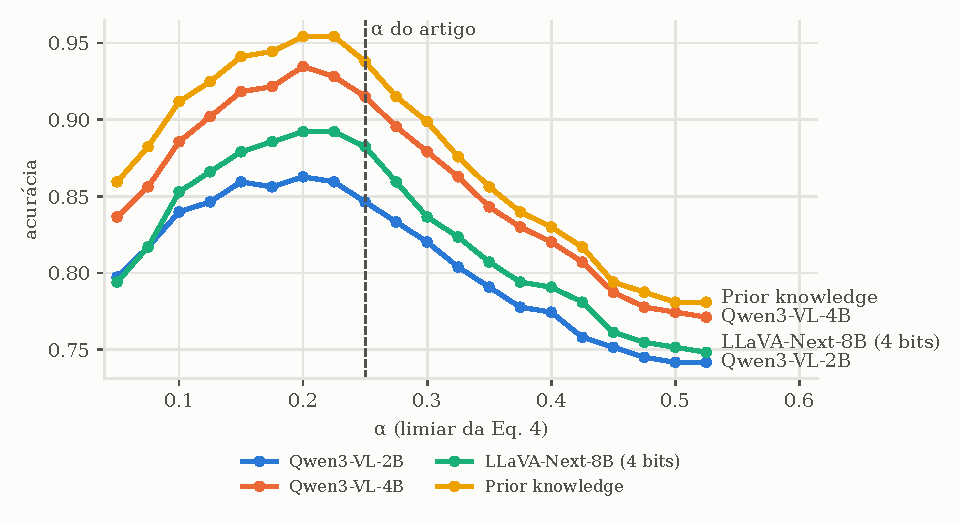
\includegraphics[width=0.78\linewidth]{fig_alpha.pdf}
\caption{Acurácia da detecção de obstrução em função do limiar $\alpha$ da Eq.~\eqref{eq:obs}
(ViDDAR com cada VLM e \emph{prior knowledge}). A linha tracejada marca o valor do artigo
($\alpha=0{,}25$). Os valores estão em \texttt{figures/fig\_alpha.csv}.}
\label{fig:alpha}
\end{figure}

\subsection{Manipulação de informação}
A Tabela~\ref{tab:man} resume os resultados. O LLaVA-Next-8B reproduz o artigo: 38,6\% de acurácia,
37,0\% de precisão e 84,1\% de recall, contra 43,0\%, 39,8\% e 95,4\% publicados. Nenhum modelo local
se aproxima do GPT-4o. Os três modelos têm acurácia de 38,6\% a 61,4\%, mas com comportamentos opostos,
que a Fig.~\ref{fig:fatores} decompõe por fator.

\begin{table}[!t]
\renewcommand{\arraystretch}{1.15}
\caption{Detecção de manipulação de informação nos 114 pares (44 com ataque), em \%}
\label{tab:man}
\centering
\footnotesize
\begin{tabular}{lcccccc}
\toprule
Modelo & Acurácia & IC 95\% & Precisão & Recall & FPR & Q6 coerente com Q3--Q5 \\
\midrule
Qwen3-VL-2B        & 38,6 & [30,2; 47,8] & 38,2 & 97,7 & \textbf{97,1} & 1,8 \\
Qwen3-VL-4B        & 61,4 & [52,2; 69,8] & 50,0 & 6,8  & 4,3  & 100 \\
LLaVA-8B (4 bits)  & 38,6 & [30,2; 47,8] & 37,0 & 84,1 & \textbf{90,0} & 100 \\
\midrule
Artigo: LLaVA-8B   & 42,98 & -- & 39,80 & 95,35 & -- & -- \\
Artigo: GPT-4o     & 82,46 & -- & 74,00 & 84,09 & 18,6$^{*}$ & -- \\
\bottomrule
\multicolumn{7}{l}{$^{*}$Derivada por nós das métricas publicadas (única matriz de confusão compatível: 37 VP, 13 FP, 57 VN, 7 FN).}
\end{tabular}
\end{table}

\begin{figure}[!t]
\centering
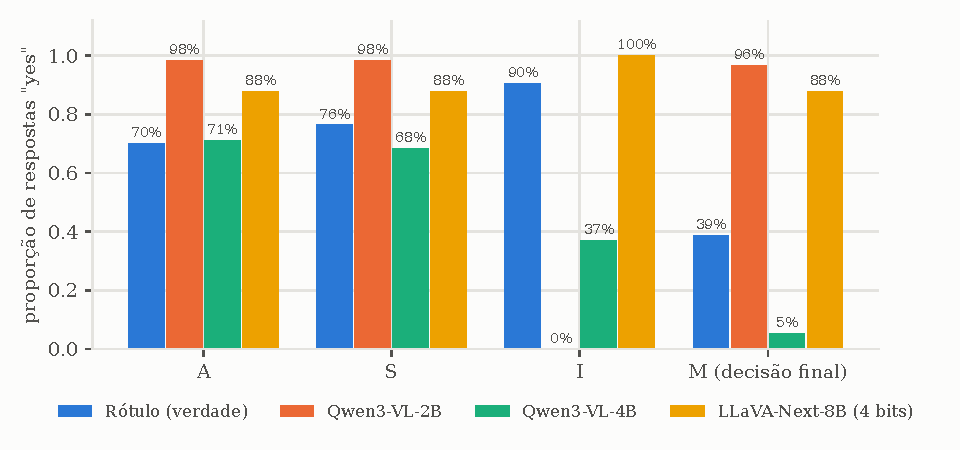
\includegraphics[width=0.78\linewidth]{fig_factors.pdf}
\caption{Proporção de respostas ``yes'' para cada fator da Eq.~\eqref{eq:man} e para a decisão final:
rótulos verdadeiros e cada VLM. O Qwen3-VL-2B nega o fator $I$ em todos os casos, mas conclui ``yes''
em 96\%; o LLaVA aceita $I$ sempre; o Qwen3-VL-4B quase nunca aceita. Os valores estão em
\texttt{figures/fig\_factors.csv}.}
\label{fig:fatores}
\end{figure}

\subsection{Exemplos de falso positivo}
A Fig.~\ref{fig:exobs} mostra um falso positivo do ViDDAR de obstrução com o Qwen3-VL-2B. O modelo
respondeu ``red box'', copiando o exemplo do próprio prompt, em vez de nomear a tomada (o objeto-chave).
Isso aconteceu em 36 das 306 imagens. O objeto detectado com esse nome estava coberto pelo conteúdo
virtual, então o sistema acusou obstrução de algo que não era o objeto-chave. Todos os 11 falsos
positivos desse modelo têm objeto-chave errado (IoU com a máscara verdadeira abaixo de 0,5).

A Fig.~\ref{fig:exman} mostra um falso positivo de manipulação com o LLaVA-Next-8B. O rótulo é negativo
porque a planta virtual flutua acima da caixa de som ($A=0$). O modelo, porém, descreveu como conteúdo
virtual o relógio exibido na tela do iPad usado como marcador de calibração, que é um objeto real, e
concluiu que havia manipulação. É o mesmo mecanismo que a hipótese prevê para placas degradadas: um
elemento real atribuído ao conteúdo virtual.

\begin{figure}[!t]
\centering
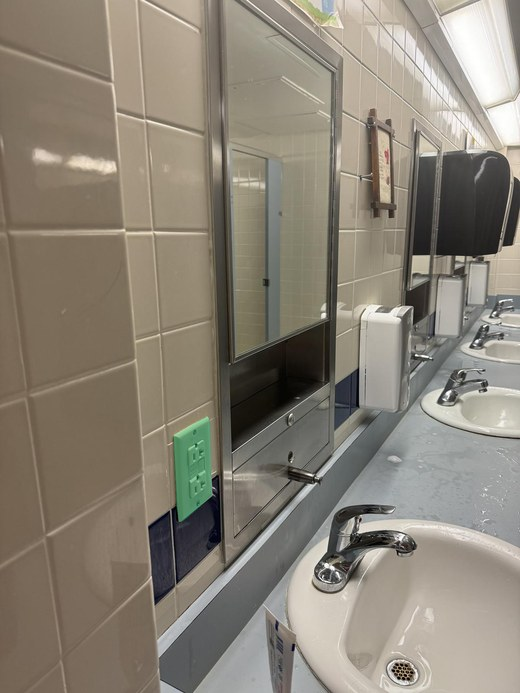
\includegraphics[width=0.26\linewidth]{ex_obs_key.jpg}\hspace{0.02\linewidth}%
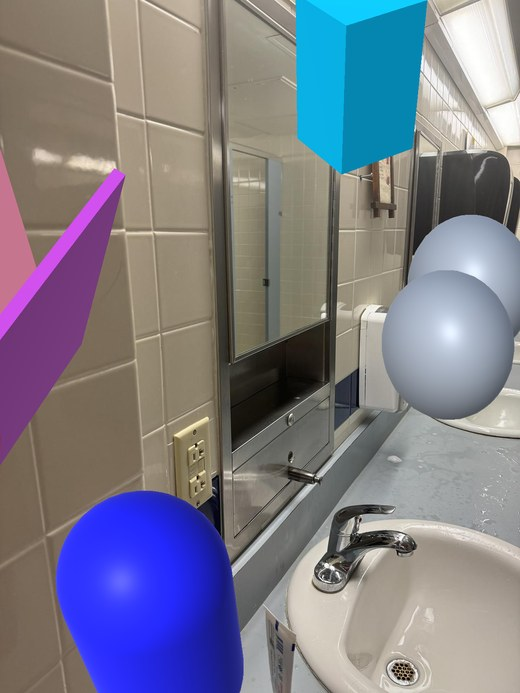
\includegraphics[width=0.26\linewidth]{ex_obs_ar.jpg}\hspace{0.02\linewidth}%
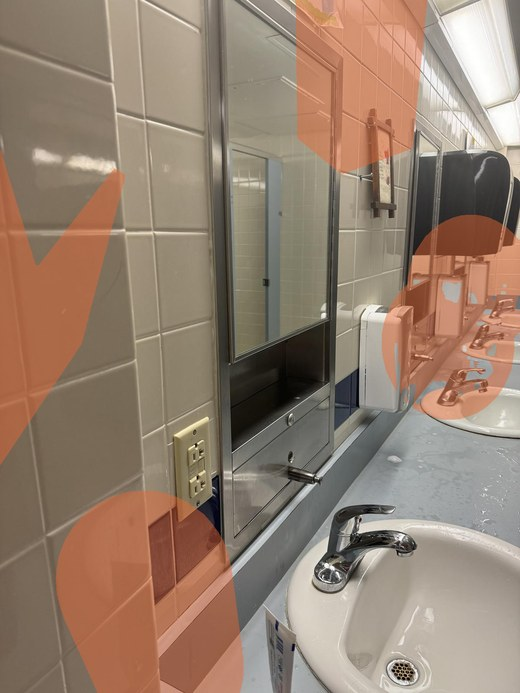
\includegraphics[width=0.26\linewidth]{ex_obs_content.jpg}
\caption{Falso positivo de obstrução (Qwen3-VL-2B, par \texttt{electrical-outlet\_004}). (a)
Esquerda: imagem crua com o objeto-chave verdadeiro (tomada) em verde. (b) Centro: imagem aumentada.
(c) Direita: máscara do conteúdo virtual em laranja. O VLM respondeu ``red box'', exemplo copiado do
prompt; a razão de obstrução do objeto detectado foi 0,45, e o IoU entre a máscara detectada e a
verdadeira foi 0,00.}
\label{fig:exobs}
\end{figure}

\begin{figure}[!t]
\centering
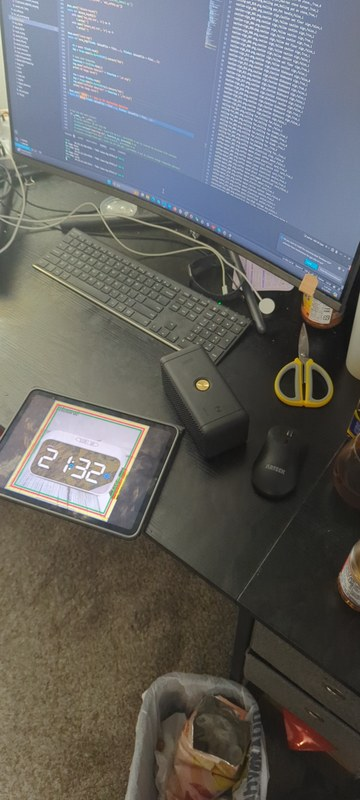
\includegraphics[width=0.24\linewidth]{ex_man_raw.jpg}\hspace{0.03\linewidth}%
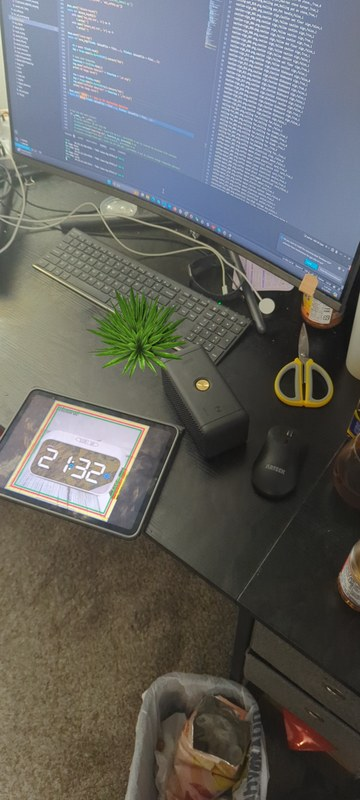
\includegraphics[width=0.24\linewidth]{ex_man_ar.jpg}
\caption{Falso positivo de manipulação (LLaVA-Next-8B, par 2). Esquerda: imagem crua. Direita: imagem
aumentada, com uma planta virtual desalinhada da caixa de som (rótulo $A=0$, $M=0$). A resposta do
modelo começa com ``The virtual content in the augmented image is a digital clock\dots'': ele tomou o
relógio da tela do iPad, real, como conteúdo virtual.}
\label{fig:exman}
\end{figure}

% =====================================================================================================
\section{Caracterização do dataset vwise}
\label{sec:dados}

Esta seção analisa o conjunto de dados disponibilizado pelo professor para o projeto (pasta
\texttt{vwise\_final}).

\subsection{Estrutura e volume}
O conjunto ocupa está organizado em 44 pastas (chamadas de recortes), cada uma correspondendo a um vídeo de origem. 
Cada pasta contém \emph{segmentos}: trechos curtos do
vídeo de origem. Ao todo há \textbf{521 segmentos}, e cada um traz:
\begin{itemize}
\item um vídeo MP4 de poucos segundos;
\item cinco quadros PNG extraídos do próprio vídeo;
\item um arquivo de rótulo (\texttt{legenda.txt}) e, em 77 segmentos, um arquivo de correção
  (\texttt{ground\_truth.txt}), descritos na Seção~\ref{sec:dados:rotulos}.
\end{itemize}
São, portanto, 2.605 quadros. A resolução varia: 1280$\times$720 (421 segmentos),
596$\times$336 (73), 1920$\times$1080 (15) e 898$\times$506 (12), com taxas de 24 a 50 quadros por
segundo. 

\subsection{Rótulos: tipo de ambiente, não placas}
\label{sec:dados:rotulos}
O rótulo não descreve placas, ele classifica o \textbf{tipo de ambiente} da cena em seis classes
(Tabela~\ref{tab:rotulos}). A Fig.~\ref{fig:vwclasses} mostra um exemplo de cada classe.

O arquivo de correção só existe onde o rótulo está errado: nos 77 segmentos que o têm (14,8\%), ele
nunca coincide com o rótulo original. Isso sugere que o rótulo original é a predição de algum
classificador automático e que a correção é humana; essa interpretação é nossa e precisa ser
confirmada.

\begin{table}[!t]
\renewcommand{\arraystretch}{1.15}
\caption{Classes de ambiente: número de segmentos pelo rótulo original e pelo rótulo efetivo (após
correções)}
\label{tab:rotulos}
\centering
\footnotesize
\begin{tabular}{lcc}
\toprule
Classe & Rótulo original & Rótulo efetivo \\
\midrule
Dirt or service road (estrada de terra/serviço) & 143 & 131 \\
Highway (rodovia) & 161 & 124 \\
Low-density urban street (rua urbana) & 95 & 97 \\
Port or dock area (área portuária) & 86 & 86 \\
High-density urban avenue (avenida densa) & 12 & 59 \\
Factory interior (interior de fábrica) & 24 & 24 \\
\midrule
Total & 521 & 521 \\
\bottomrule
\end{tabular}
\end{table}

\begin{figure}[!t]
\centering
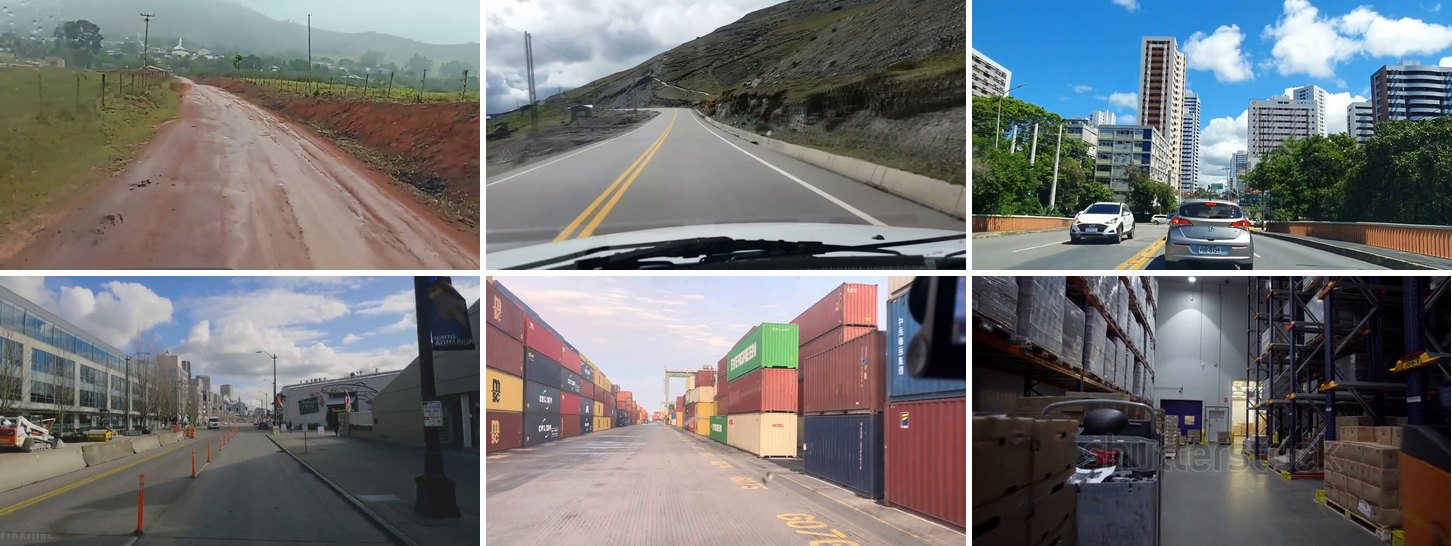
\includegraphics[width=0.82\linewidth]{vw_classes.jpg}
\caption{Um quadro de cada classe de ambiente. Linha de cima: estrada de terra, rodovia e rua urbana
de baixa densidade. Linha de baixo: avenida densa, área portuária e interior de fábrica.}
\label{fig:vwclasses}
\end{figure}

\subsection{Origem das imagens}
Inspecionando segmentos diferentes de cada vídeo de origem, identificamos três grupos:
\begin{itemize}
\item \textbf{Gravações de direção} (25 vídeos, 381 segmentos, 1280$\times$720): câmera no painel ou
  no para-brisa de carros e caminhões, no estilo de vídeos publicados no YouTube. Vários trazem
  elementos de interface do vídeo, como o logo de um canal, o botão ``INSCREVA-SE'',
  cronômetros e legendas.
\item \textbf{Vídeos de banco de imagens} (17 vídeos, 87 segmentos): 15 deles, em baixa resolução
  (596$\times$336 ou 898$\times$506), têm marca d'água ``shutterstock''; os outros 2, em 1080p e sem
  marca, mostram um terminal de grãos. Mostram armazéns, portos e rodovias; 7 desses vídeos têm um
  único segmento, e 13 segmentos nem são vistos de um veículo (trabalhadores parados, interior de
  contêiner).
\item \textbf{Outros} (2 vídeos, 53 segmentos): gravações urbanas.
\end{itemize}

\subsection{Localidade}
A proposta pressupunha imagens da América Latina. Alguns vídeos parecem de fato
da América Latina, pois há placas em português e em espanhol (Fig.~\ref{fig:vwsigns}). No entanto,
\textbf{encontramos vários exemplos de cenas gravadas fora da América Latina}
(Fig.~\ref{fig:vwlocal}): placas de rodovia e de terminais portuários dos EUA, sinalização em milhas
por hora, placas em japonês, placa de advertência no padrão europeu e vagões com inscrições em
cirílico. Além disso, vários vídeos de banco de imagens (armazéns, portos) não trazem nenhuma pista do
local (nem placas de trânsito).

Como o conjunto não traz anotação de localidade e o local só pode ser inferido quando há pistas
visuais, não é possível quantificar com segurança quanto do conjunto vem de cada região. A conclusão
relevante para a proposta é qualitativa: \textbf{o conjunto não é exclusivamente latino-americano}, e
um estudo restrito à América Latina exigiria antes um trabalho de curadoria para filtrar os vídeos.

\begin{figure}[!t]
\centering
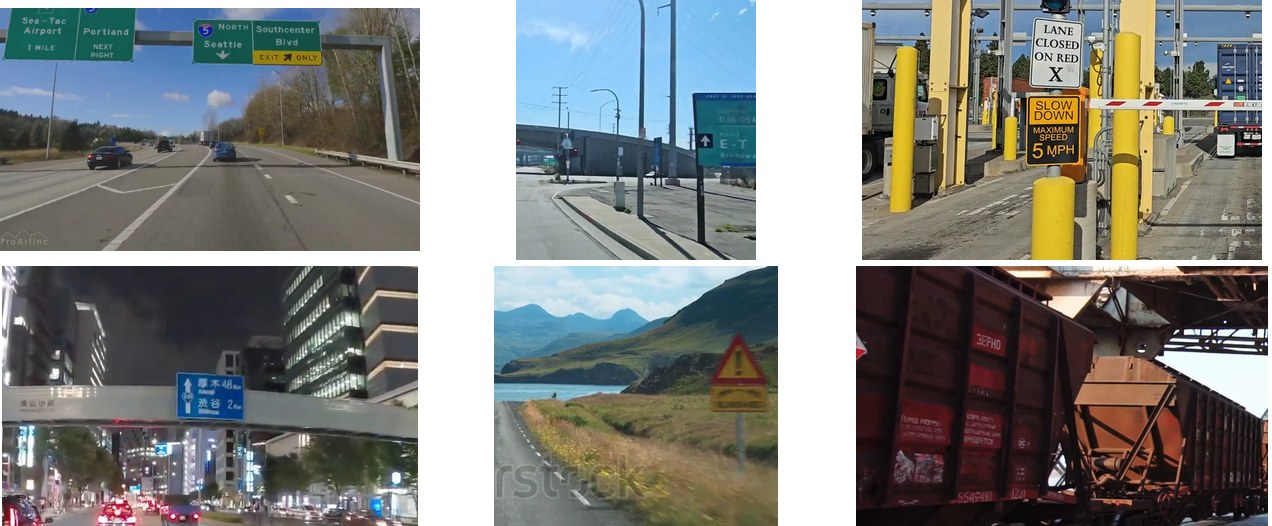
\includegraphics[width=0.82\linewidth]{vw_locality.jpg}
\caption{Exemplos de cenas gravadas fora da América Latina. Linha de cima: placas de rodovia em
Seattle (EUA), placa do Porto de Long Beach (EUA) e sinalização em milhas por hora em um terminal
portuário. Linha de baixo: placa de direção em japonês (Tóquio), placa de advertência no padrão europeu
e vagões com a palavra russa \emph{zerno} (``grão'') escrita em cirílico.}
\label{fig:vwlocal}
\end{figure}


\subsection{Sobreposições já presentes nos vídeos}
\label{sec:dados:overlays}
Um achado relevante para RA é que \textbf{pelo menos 23 dos 44 vídeos de origem (212 segmentos,
40,7\%) já contêm sobreposições 2D}, gravadas na própria imagem (Fig.~\ref{fig:vwoverlays}): marcas
d'água (``shutterstock'' de banco de imagens), logos
de canal, elementos de interface do YouTube, cronômetros e legendas em português, inglês e japonês.
Do ponto de vista de um detector de RA, são conteúdos artificiais sobre a cena real que estão presentes
tanto em $\Ir$ quanto em qualquer $\Ia$ gerada a partir dela.

\begin{figure}[!t]
\centering
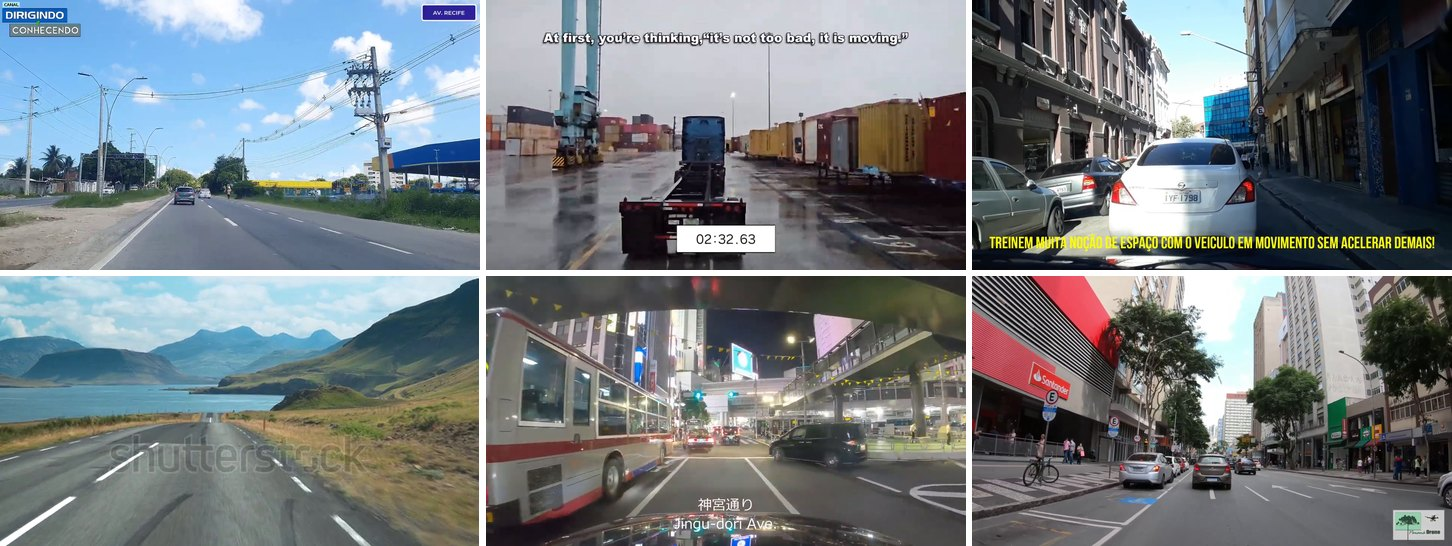
\includegraphics[width=0.82\linewidth]{vw_overlays.jpg}
\caption{Sobreposições gravadas nos próprios vídeos. Linha de cima: logo de canal e nome da via,
cronômetro e legenda em inglês, legenda em português (vídeo de autoescola). Linha de baixo: marca
d'água ``shutterstock'', legenda com o nome da via em japonês e logo de canal no canto inferior
direito.}
\label{fig:vwoverlays}
\end{figure}

\subsection{Placas: quantas existem e em que estado}
\label{sec:dados:placas}
O conjunto não traz anotação de placas. Para estimar sua presença, aplicamos aos 2.605 quadros o mesmo
detector do pipeline, o Grounding DINO, com a consulta ``traffic sign'' (Tabela~\ref{tab:deteccao}).
\textbf{O detector encontra poucas placas}: com confiança $\geq 0{,}45$, só 137 dos 521 segmentos
(26\%) têm alguma detecção em pelo menos um quadro, e com $\geq 0{,}55$, apenas 42 (8\%). As detecções
se concentram nas rodovias; nos interiores de fábrica não há nenhuma.

Esses números são limites superiores, porque nem toda detecção é uma placa: o detector também dispara
em adesivos no painel, no limpador de para-brisa, em logos e cronômetros sobrepostos ao vídeo, em
contêineres e em cones (Fig.~\ref{fig:vwsigns}, linha de baixo). Além disso, as placas detectadas são
\textbf{pequenas}: a maior detecção de cada quadro ocupa, na mediana, 0,6\% da área do quadro, e muitas
estão borradas por movimento, chuva ou baixa resolução.

A Fig.~\ref{fig:vwsigns} também mostra que as placas presentes são de \textbf{origens e idiomas
diversos}: português, espanhol, inglês e japonês, em padrões de sinalização de países diferentes. Nessa
resolução, não é possível avaliar o estado físico das placas (desgaste, pichação, adesivos).

\begin{table}[!t]
\renewcommand{\arraystretch}{1.15}
\caption{Porcentagem de segmentos e de quadros com detecção de placa pelo Grounding DINO, por limiar
de confiança}
\label{tab:deteccao}
\centering
\footnotesize
\begin{tabular}{lccc}
\toprule
 & Conf. $\geq 0{,}35$ & Conf. $\geq 0{,}45$ & Conf. $\geq 0{,}55$ \\
\midrule
Segmentos (521) & 55,5\% & 26,3\% & 8,1\% \\
Quadros (2.605) & 30,7\% & 11,0\% & 3,3\% \\
\bottomrule
\end{tabular}
\end{table}

\begin{figure}[!t]
\centering
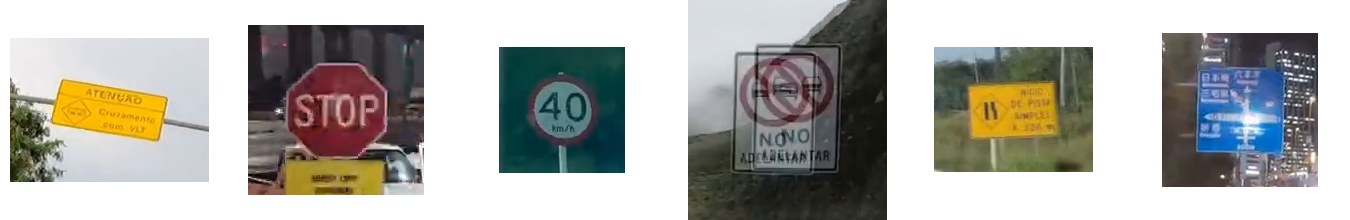
\includegraphics[width=0.86\linewidth]{vw_signs_real.jpg}\\[3pt]
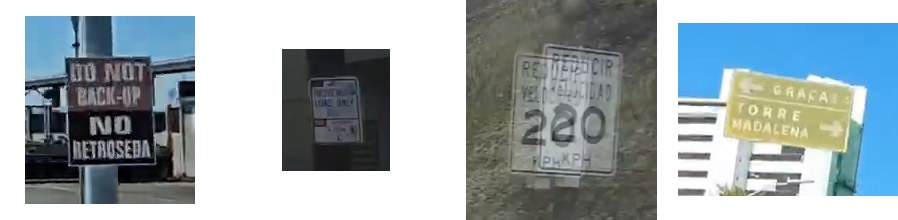
\includegraphics[width=0.58\linewidth]{vw_signs_degraded.jpg}\\[3pt]
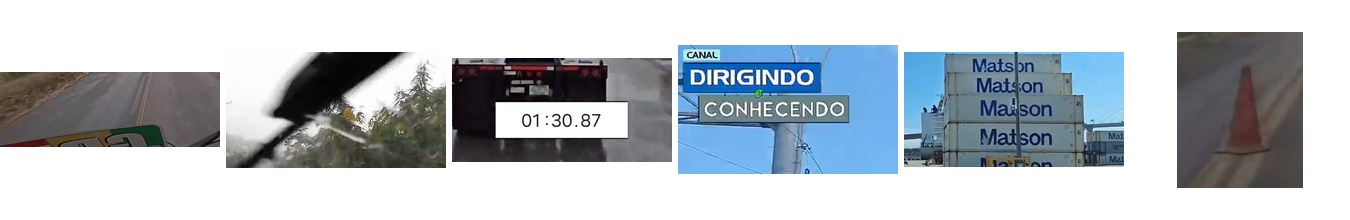
\includegraphics[width=0.86\linewidth]{vw_signs_fp.jpg}
\caption{Exemplos de detecções do Grounding DINO. Linha de cima: placas em diferentes idiomas e
padrões (português, inglês, espanhol e japonês). Linha do meio: outras placas detectadas, pequenas ou
borradas; nessa resolução não é possível avaliar o estado físico. Linha de baixo: detecções que não
são placas (adesivo no painel, limpador, cronômetro sobreposto, logo de canal, contêineres e cone).}
\label{fig:vwsigns}
\end{figure}


% =====================================================================================================
\section{Discussão}
\label{sec:disc}

\subsection{A replicação é confiável}
Os componentes sem VLM reproduzem o artigo quase exatamente, e o mesmo VLM do artigo produz números
próximos dos publicados em todos os métodos. Portanto, diferenças que observarmos nos dados do projeto
poderão ser atribuídas aos dados, e não a erros de reimplementação. A troca do Grounding DINO 1.5 pela
versão aberta não prejudicou a segmentação (mIoU de 85,1\% contra 78,8\% no \emph{prior knowledge}).

\subsection{Implicações da replicação para a proposta}
\textbf{Obstrução.} A FPR baixa do ViDDAR (3,7\% a 6,8\%) deixa margem para medir um aumento causado
pela degradação. Como argumentado na Seção~\ref{sec:metodo}, esperamos que esse aumento venha
sobretudo da escolha do objeto-chave. O exemplo ``red box'' mostra que erros de reconhecimento já
geram falsos positivos mesmo em dados limpos.

\textbf{Manipulação.} Com FPR de 90\% a 97\% já nos dados curados, o Qwen3-VL-2B e o LLaVA não deixam
espaço para medir um aumento causado pela degradação: o efeito ficaria escondido pelo teto. O
Qwen3-VL-4B tem o problema oposto. Com FPR de 4\% e recall de 7\%, ele quase nunca dispara, e uma FPR
baixa não significaria robustez. Para a hipótese ser testável, precisamos de um modelo aberto com ponto
de operação equilibrado nos dados originais, próximo do que o artigo obteve com o GPT-4o (FPR de 18,6\%
e recall de 84,1\%). Nenhum dos três modelos testados atende a esse requisito.

\textbf{Mecanismos de erro.} Lembrando o funcionamento do questionário: as perguntas 3, 4 e 5 pedem ao
VLM que julgue $A$, $S$ e $I$, e a pergunta 6 pede a conclusão, instruindo-o a responder ``yes'' somente
se respondeu ``yes'' às três anteriores. A decisão oficial do ViDDAR é a conclusão (pergunta 6). Como
guardamos também as respostas 3--5, podemos verificar se a conclusão de cada modelo é coerente com
os próprios julgamentos e qual fator ele erra. Os três modelos têm acurácias parecidas, mas erram por
motivos diferentes (Fig.~\ref{fig:fatores}):
\begin{itemize}
\item \emph{Incoerência lógica} (Qwen3-VL-2B). O modelo responde ``no'' ao fator $I$ em todos os pares
  em que a resposta pôde ser interpretada. Pelas próprias respostas, a conclusão deveria ser sempre
  ``no''; mesmo assim, ele conclui ``yes'' em 96\% dos pares, muitas vezes afirmando que respondeu
  ``yes'' às perguntas 3, 4 e 5. A conclusão só é coerente com as respostas anteriores em 1,8\% dos
  casos. Se a decisão fosse tomada pela Eq.~\eqref{eq:man} a partir das respostas 3--5, a FPR cairia
  de 97\% para 0\%, mas o recall também iria a 0\%: o modelo deixaria de detectar qualquer ataque. Os
  falsos positivos desse modelo vêm, portanto, da etapa de conclusão, e não de uma leitura da cena.
\item \emph{Credulidade} (LLaVA-Next-8B). A conclusão é sempre coerente com as respostas 3--5, mas o
  modelo aceita quase tudo: responde ``yes'' ao fator $I$ em 100\% dos pares e a $A$ e $S$ em 88\%,
  contra 90\%, 70\% e 76\% nos rótulos. Como quase todo par satisfaz $A\wedge S\wedge I$ segundo o
  modelo, quase todo par vira manipulação (FPR de 90\%).
\item \emph{Ceticismo} (Qwen3-VL-4B). Também coerente, mas aceita o fator $I$ em apenas 37\% dos pares
  (90\% nos rótulos). Raramente os três fatores são aceitos juntos, e o modelo conclui ``yes'' em só 5\%
  dos pares: FPR de 4\%, mas recall de 7\%.
\end{itemize}

\subsection{Viabilidade da proposta com os dados disponíveis}
\label{sec:viabilidade}
A caracterização da Seção~\ref{sec:dados} permite avaliar a proposta ponto a ponto:
\begin{itemize}
\item \textbf{Formato: compatível.} As imagens são reais, sem conteúdo virtual, e vêm em vídeos com
  quadros extraídos. O pipeline do ViDDAR roda sobre os quadros sem modificação, desde que as imagens
  aumentadas sejam geradas sinteticamente, como já previsto. O formato em vídeo também abre a
  possibilidade de usar o VIM-Sense.
\item \textbf{Placas degradadas: insuficientes.} A hipótese original depende de placas fisicamente
  degradadas. O detector encontra placas em no máximo cerca de um quarto dos segmentos, contando
  detecções que não são placas; elas são pequenas e muitas vezes borradas, e não exibem degradação
  física evidente. Isso está longe dos cerca de 140 pares por grupo estimados na
  Seção~\ref{sec:metodo}. \textbf{A hipótese, como formulada, não pode ser testada só com estes dados.}
\item \textbf{Localidade: mista.} Há placas em português e espanhol, mas também vários exemplos de
  fora da América Latina (Fig.~\ref{fig:vwlocal}), e o local não é anotado.
\end{itemize}
Com base nisso, vemos dois caminhos:
\begin{enumerate}
\item \textbf{Obter dados com placas degradadas.} Se existir outro conjunto (por exemplo, do próprio
  Voxar Labs) com placas degradadas anotadas da América Latina, a metodologia da Seção~\ref{sec:metodo} se aplica
  diretamente. É o caminho mais fiel à proposta desse relatório.
\item \textbf{Alternativa: benchmark de VLMs com os dados do próprio ViDDAR.} Como alternativa
podemos voltar para a nossa proposta original, antes do professor sugerir o dataset de placas. Retomar os dados do
  ViDDAR e fazer deles o objeto principal: um
  benchmark de VLMs de código aberto na detecção de conteúdo prejudicial em RA. Os dados já estão rotulados 
  (306 pares de obstrução e 114 de manipulação), e o pipeline de
  avaliação está reconstruído e validado (Seção~\ref{sec:exp}).
  A vantagem é poder começar imediatamente, sem coleta ou anotação de dados. A desvantagem é que o
  estudo deixa de tratar de placas degradadas e de condições realistas.
\end{enumerate}
O caminho 1 preserva a proposta descrita nesse documento, mas depende da existência de outro conjunto de dados. O
caminho 2 pode ser executado com o que já temos. A decisão depende das respostas às questões da
Seção~\ref{sec:aberto}.

% =====================================================================================================
\section{Limitações}
\begin{itemize}
\item Os VLMs testados são pequenos (2B a 8B), e o LLaVA está quantizado em 4 bits. O artigo usou o
  LLaVA completo, via API.
\item Os resultados vêm de uma única execução com decodificação determinística; não estimamos ainda a
  variância entre execuções, que o próprio artigo aponta como fonte de instabilidade.
\item O artigo não publica o critério de acerto do objeto-chave. Usamos dois critérios próprios
  (léxico e por sobreposição de máscara), então essa métrica não é diretamente comparável.
\item Por decisão do projeto, usamos apenas modelos de código aberto. Não há, portanto, comparação
  direta com o GPT-4o, modelo principal do artigo, além dos números publicados.
\item Latência, o app de RA e o estudo com usuários do artigo estão fora do escopo.
\item As imagens aumentadas do experimento principal serão sintéticas (composição 2D). Isso dá
  controle total, mas pode reduzir o realismo do conteúdo virtual em relação a uma captura em RA real.
\item \textbf{(Draft 2)} A presença de placas foi estimada por detecção automática, que inclui
  detecções que não são placas e não avalia o estado físico. A localidade não é anotada no conjunto e
  só pode ser inferida quando há pistas visuais.
\end{itemize}

% =====================================================================================================
\section{Questões em aberto e próximos passos}
\label{sec:aberto}

\subsection{Respondidas}
\begin{itemize}
\item \textbf{Formato dos dados:} vídeos de cerca de 10~s com cinco quadros extraídos cada; tanto o
  ViDDAR (quadros) quanto o VIM-Sense (vídeos) são aplicáveis.
\item \textbf{Volume e anotações:} 521 segmentos, rotulados por tipo de ambiente; não há anotação de
  placas, de degradação nem de localidade (Seção~\ref{sec:dados}).
\end{itemize}

\subsection{A confirmar com o professor}
\begin{enumerate}
\item \textbf{É este o conjunto de placas mencionado na proposta?} Ou existe outro, com placas
  degradadas da América Latina?
\item \textbf{Direção do trabalho:} se não houver outro conjunto de dados (caminho 1 da
  Seção~\ref{sec:viabilidade}), o benchmark de VLMs com os dados do próprio ViDDAR (caminho 2) é
  aceitável como objeto de estudo?
\item \textbf{Significado dos rótulos:} de qual classificador vem o rótulo original, e se as
  correções são de fato humanas.
\item \textbf{Uso das imagens:} parte dos vídeos é de banco de imagens com marca d'água e parte é de
  canais do YouTube. Convém confirmar se podemos reproduzir quadros em publicações.
\item \textbf{Escopo das mitigações:} confirmar se o trabalho se limita aos detectores sem
  modificações ou se inclui variantes de prompt.
\end{enumerate}

\subsection{O que ainda falta validar}
\begin{enumerate}
\item \textbf{Escolha do VLM para manipulação:} testar VLMs de código aberto maiores que caibam na GPU
  com quantização em 4 bits (por exemplo, Qwen3-VL-8B) e verificar se algum atinge, nos dados
  originais, um ponto de operação equilibrado, próximo ao do GPT-4o no artigo. Se nenhum atingir,
  avaliar como complemento a decisão pela Eq.~\eqref{eq:man} calculada a partir das respostas 3--5,
  reportada sempre ao lado da decisão original do ViDDAR.
\item \textbf{Variância:} repetir execuções com amostragem estocástica para estimar a variação das
  métricas.
\item \textbf{Conjunto de modelos do benchmark (caminho 2):} definir quais VLMs abertos entram, por
  família e tamanho, e as variantes de prompt avaliadas.
\item \textbf{Limiar $\alpha$:} decidir se reportamos com $\alpha=0{,}25$ (artigo) ou $0{,}2$ (mais
  coerente com os rótulos), mantendo sempre ambos.
\item \textbf{Pares sintéticos (caminho 1):} se houver um conjunto com placas degradadas, anotar as
  placas que ele não trouxer anotadas (caixa e máscara via SAM), implementar a composição das condições
  C0--C4 e verificar que o pipeline produz as decisões esperadas em placas íntegras: FPR baixa em C0--C2
  e detecção em C3--C4. Os rótulos de C4 (manipulação) dependem de julgamento humano; planejamos
  validá-los em pequena escala, nos moldes do estudo com usuários do artigo.
\end{enumerate}

% =====================================================================================================
\section{Conclusão}
Reconstruímos e validamos o pipeline de avaliação do ViDDAR, cujo código público era incompleto, com
VLMs locais. Com o mesmo VLM do artigo, a replicação reproduz os resultados publicados, e um modelo de
4B parâmetros praticamente iguala o GPT-4o na detecção de obstrução. A replicação também mostrou que a
decisão geométrica do ViDDAR de obstrução deve ser pouco sensível à degradação, ao contrário dos
componentes em que o VLM julga diretamente, e que, na detecção de manipulação, a escolha do VLM é
decisiva, porque modelos pequenos já operam perto de 100\% ou de 0\% de respostas positivas.

Neste segundo rascunho, a caracterização dos dados do projeto mostrou que eles são vídeos de direção
rotulados por tipo de ambiente, não um dataset de placas. O detector encontra poucas placas, em geral
pequenas e pouco nítidas, em idiomas variados, sem degradação física evidente, e o conjunto inclui
vários exemplos gravados fora da América Latina. Com esses dados, a hipótese original não pode ser
testada diretamente. Vemos dois caminhos: obter outro conjunto com placas degradadas anotadas, o que
preserva a proposta original, ou, como alternativa, usar os dados do próprio ViDDAR para um benchmark
de VLMs abertos com foco em falsos positivos, aproveitando o pipeline já validado. Submetemos essa
decisão ao professor.

% =====================================================================================================
\begin{thebibliography}{99}

\bibitem{viddar}
Y.~Xiu, T.~Scargill, and M.~Gorlatova, ``{ViDDAR}: Vision language model-based task-detrimental
content detection for augmented reality,'' \emph{IEEE Trans. Vis. Comput. Graphics}, vol.~31, no.~5,
pp. 3194--3203, 2025, doi: 10.1109/TVCG.2025.3549147.

\bibitem{vimsense}
Y.~Xiu and M.~Gorlatova, ``Detecting visual information manipulation attacks in augmented reality: A
multimodal semantic reasoning approach,'' \emph{IEEE Trans. Vis. Comput. Graphics}, 2025, preprint
arXiv:2507.20356.

\bibitem{hendrycks2019}
D.~Hendrycks and T.~Dietterich, ``Benchmarking neural network robustness to common corruptions and
perturbations,'' in \emph{Proc. Int. Conf. Learn. Represent. (ICLR)}, 2019.

\bibitem{hendrycks2021}
D.~Hendrycks, K.~Zhao, S.~Basart, J.~Steinhardt, and D.~Song, ``Natural adversarial examples,'' in
\emph{Proc. IEEE/CVF Conf. Comput. Vis. Pattern Recognit. (CVPR)}, 2021, pp. 15262--15271.

\bibitem{eykholt2018}
K.~Eykholt \emph{et al.}, ``Robust physical-world attacks on deep learning visual classification,''
in \emph{Proc. IEEE/CVF Conf. Comput. Vis. Pattern Recognit. (CVPR)}, 2018, pp. 1625--1634.

\bibitem{groundingdino}
S.~Liu \emph{et al.}, ``Grounding {DINO}: Marrying {DINO} with grounded pre-training for open-set
object detection,'' in \emph{Proc. Eur. Conf. Comput. Vis. (ECCV)}, 2024, preprint arXiv:2303.05499.

\bibitem{sam}
A.~Kirillov \emph{et al.}, ``Segment anything,'' in \emph{Proc. IEEE/CVF Int. Conf. Comput. Vis.
(ICCV)}, 2023, pp. 4015--4026.

\bibitem{llava}
H.~Liu, C.~Li, Q.~Wu, and Y.~J. Lee, ``Visual instruction tuning,'' in \emph{Adv. Neural Inf.
Process. Syst. (NeurIPS)}, vol.~36, 2023.

\bibitem{qwen3vl}
Qwen Team, ``{Qwen3-VL} model cards (2B and 4B Instruct),'' Hugging Face, 2025. [Online]. Available:
\url{https://huggingface.co/Qwen/Qwen3-VL-4B-Instruct}

\bibitem{qlora}
T.~Dettmers, A.~Pagnoni, A.~Holtzman, and L.~Zettlemoyer, ``{QLoRA}: Efficient finetuning of
quantized {LLMs},'' in \emph{Adv. Neural Inf. Process. Syst. (NeurIPS)}, vol.~36, 2023.

\bibitem{hou2007}
X.~Hou and L.~Zhang, ``Saliency detection: A spectral residual approach,'' in \emph{Proc. IEEE Conf.
Comput. Vis. Pattern Recognit. (CVPR)}, 2007.

\bibitem{canny}
J.~Canny, ``A computational approach to edge detection,'' \emph{IEEE Trans. Pattern Anal. Mach.
Intell.}, vol.~PAMI-8, no.~6, pp. 679--698, 1986.

\bibitem{wilson}
E.~B. Wilson, ``Probable inference, the law of succession, and statistical inference,'' \emph{J. Amer.
Statist. Assoc.}, vol.~22, no.~158, pp. 209--212, 1927.

\end{thebibliography}

\end{document}
